\begin{figure}[htbp]
\centering
\resizebox{\textwidth}{!}{%
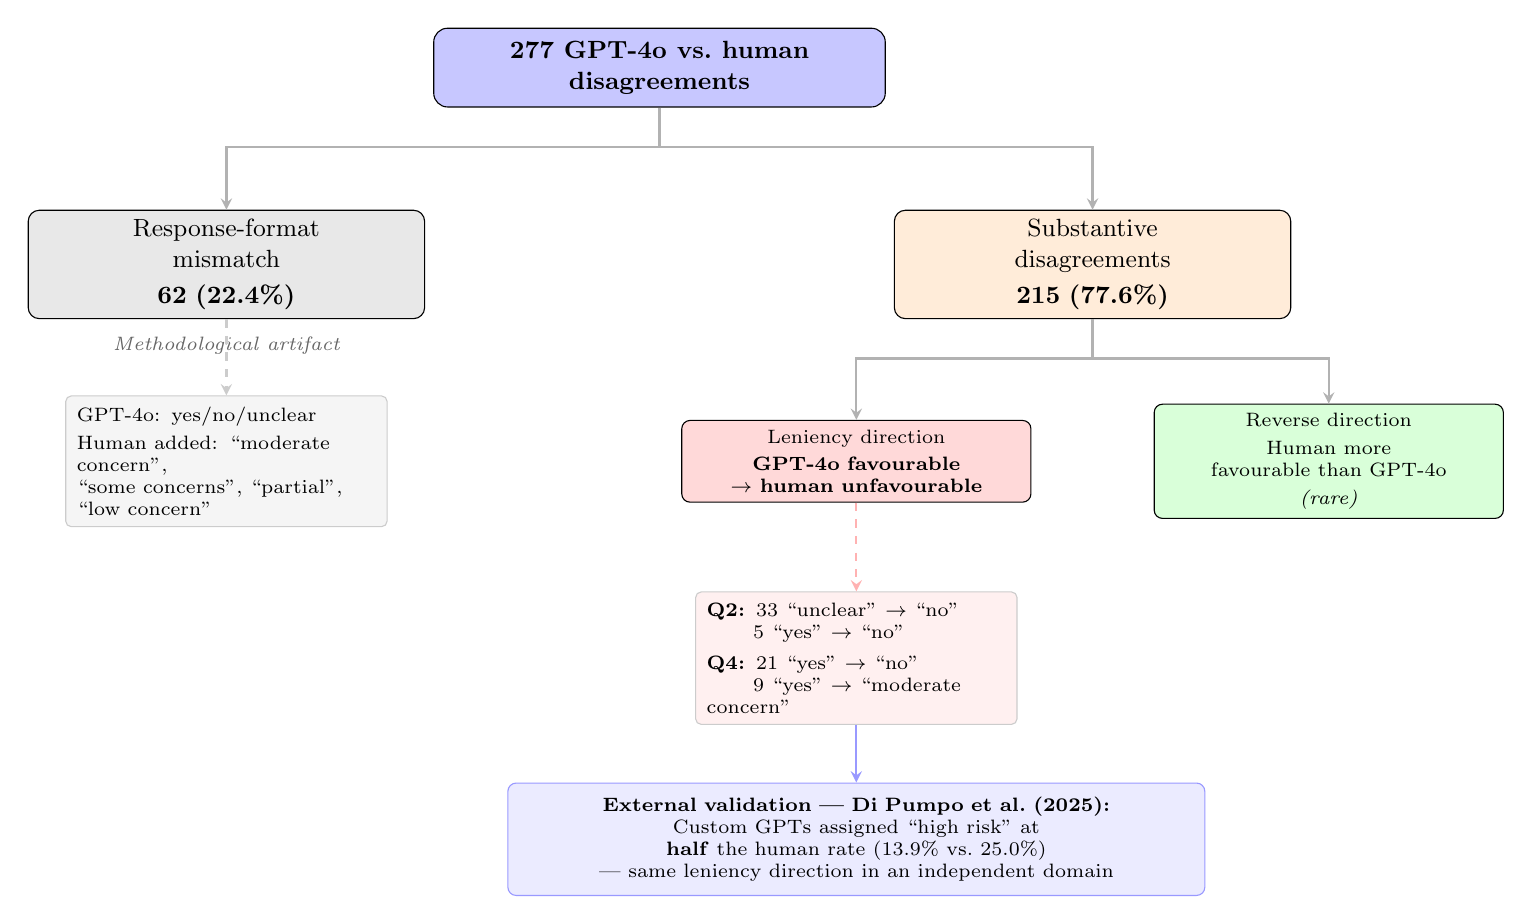
\begin{tikzpicture}[
  rootbox/.style={rectangle, draw, rounded corners=5pt, fill=blue!22,
    text width=5.5cm, minimum height=1.0cm, align=center, font=\small\bfseries},
  catbox/.style={rectangle, draw, rounded corners=4pt,
    text width=4.8cm, minimum height=0.9cm, align=center, font=\small},
  subbox/.style={rectangle, draw, rounded corners=3pt,
    text width=4.2cm, minimum height=0.8cm, align=center, font=\scriptsize},
  exbox/.style={rectangle, draw=gray!40, rounded corners=2pt, fill=white,
    text width=3.8cm, align=left, font=\scriptsize, inner sep=4pt},
  valbox/.style={rectangle, draw=blue!40, rounded corners=3pt, fill=blue!8,
    text width=8.5cm, align=center, font=\scriptsize, inner sep=5pt},
  ann/.style={font=\scriptsize\itshape, text=black!60},
  arr/.style={->, >=stealth, thick, draw=gray!60},
]

% ============================================================
% ROOT NODE
% ============================================================
\node[rootbox] (root) at (0, 0) {277 GPT-4o vs.\ human\\disagreements};

% ============================================================
% BRANCH A: Response-format mismatch
% ============================================================
\node[catbox, fill=gray!18] (fmatch) at (-5.5, -2.5) {Response-format\\mismatch\\[2pt]\textbf{62 (22.4\%)}};
\node[ann, anchor=north] at (-5.5, -3.3) {Methodological artifact};

% ============================================================
% BRANCH B: Substantive disagreements
% ============================================================
\node[catbox, fill=orange!15] (subst) at (5.5, -2.5) {Substantive\\disagreements\\[2pt]\textbf{215 (77.6\%)}};

% Arrows from root
\draw[arr] (root.south) -- ++(0, -0.5) -| (fmatch.north);
\draw[arr] (root.south) -- ++(0, -0.5) -| (subst.north);

% ============================================================
% Format mismatch detail
% ============================================================
\node[exbox, fill=gray!8] (fmdet) at (-5.5, -5.0) {%
  GPT-4o: yes/no/unclear\\[2pt]
  Human added: ``moderate concern'',\\
  ``some concerns'', ``partial'',\\
  ``low concern''};
\draw[arr, dashed, draw=gray!40] (fmatch.south) -- (fmdet.north);

% ============================================================
% BRANCH B1: Leniency direction (dominant)
% ============================================================
\node[subbox, fill=red!15] (leniency) at (2.5, -5.0) {Leniency direction\\[2pt]\textbf{GPT-4o favourable}\\$\rightarrow$ \textbf{human unfavourable}};

% ============================================================
% BRANCH B2: Reverse direction (minor)
% ============================================================
\node[subbox, fill=green!15] (reverse) at (8.5, -5.0) {Reverse direction\\[2pt]Human more\\favourable than GPT-4o\\[2pt]{\itshape(rare)}};

% Arrows from substantive
\draw[arr] (subst.south) -- ++(0, -0.5) -| (leniency.north);
\draw[arr] (subst.south) -- ++(0, -0.5) -| (reverse.north);

% ============================================================
% Leniency examples
% ============================================================
\node[exbox, fill=red!6] (lex) at (2.5, -7.5) {%
  \textbf{Q2:} 33 ``unclear'' $\rightarrow$ ``no''\\
  \hspace{2.1em}5 ``yes'' $\rightarrow$ ``no''\\[3pt]
  \textbf{Q4:} 21 ``yes'' $\rightarrow$ ``no''\\
  \hspace{2.1em}9 ``yes'' $\rightarrow$ ``moderate concern''};
\draw[arr, dashed, draw=red!30] (leniency.south) -- (lex.north);

% ============================================================
% EXTERNAL VALIDATION
% ============================================================
\node[valbox] (extval) at (2.5, -9.8) {%
  \textbf{External validation --- Di~Pumpo et al.\ (2025):}\\
  Custom GPTs assigned ``high risk'' at \textbf{half} the human rate (13.9\% vs.\ 25.0\%)\\
  --- same leniency direction in an independent domain};
\draw[arr, draw=blue!40] (lex.south) -- (extval.north);

\end{tikzpicture}%
}% end resizebox
\caption{Taxonomy of the 277 disagreements between GPT-4o and human-verified risk-of-bias assessments. Response-format mismatches (22.4\%) inflate measured disagreement without reflecting substantive differences. Among substantive disagreements, the dominant pattern is leniency bias: GPT-4o systematically applied less stringent criteria than human reviewers, consistent with independent findings by Di~Pumpo et~al.~(2025).}
\label{fig:disagreement-taxonomy}
\end{figure}
